
\hypertarget{menu_r}{}
\section{R}
\index{R menu}

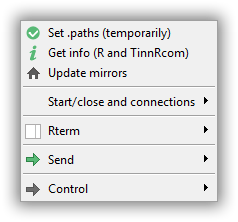
\includegraphics[scale=0.50]{./res/menu_r.png}\\

\begin{scriptsize}\begin{tabularx}{\textwidth}{>{\hsize=0.5\hsize}X>{\hsize=0.7\hsize}X}\\
    \hline
    \textbf{Option} & \textbf{Description} \\
    \hline
%    Start/close and connections & \textit{\htmladdnormallink{See options ...}{\#menu\_r\_startcloseandconections}} \\
    Set .paths (temporarily) & Sets (temporarily) the necessary .paths object in \RR{} environment
    This object provided by TinnRcom package. This option is useful only if the user can not, for some reason,   install the TinnRcom package \\
    Get info (R and TinnRcom) & Get information about \RR{} and the necessary TinnRcom package \\
    Update mirrors & Updates the Rmirrors.xml file \\
    Rterm & \textit{\htmladdnormallink{See options ...}{\#menu\_r\_rterm}} \\
    Send & \textit{\htmladdnormallink{See options ...}{\#menu\_r\_send}} \\
%    Editor: current line to top & Brings the current line to the top of the editor interface \\
    Control & \textit{\htmladdnormallink{See options ...}{\#menu\_r\_control}} \\
    \hline
  \end{tabularx}\end{scriptsize}


\hypertarget{menu_r_startcloseandconections}{}
\subsection{Start/close and connections}
\index{R menu!start}
\index{R menu!close}
\index{R menu!connections}

\includegraphics[scale=0.50]{./res/menu_r_startcloseandconections.png}\\

\begin{scriptsize}\begin{tabularx}{\textwidth}{>{\hsize=0.5\hsize}X>{\hsize=0.7\hsize}X}\\
    \hline
    \textbf{Option} & \textbf{Description} \\
    \hline
    Rterm (start/close) & Starts and Closes Rterm interface \\
    Rgui (start/close) & Starts and Closes Rgui application \\
    Server (connections and tests) & Opens the dialog \textit{R server: connections and tests} \\
    \hline
  \end{tabularx}\end{scriptsize}

Tip: the \textit{Server (connections and tests)} dialog allows you to test the
TCP/IP communication protocols used to establish a communication between
R and Tinn-R.


\hypertarget{menu_r_rterm}{}
\subsection{Rterm}
\index{R menu!Rterm}

\includegraphics[scale=0.50]{./res/menu_r_rterm.png}\\

\begin{scriptsize}\begin{tabularx}{\textwidth}{>{\hsize=0.7\hsize}X>{\hsize=0.7\hsize}X}\\
    \hline
    \textbf{Option} & \textbf{Description} \\
    \hline
    Rterm (show/hide) & Toggles (show/hide) Rterm interface \\
    File & \textit{\htmladdnormallink{See options ...}{\#menu\_r\_rterm\_file}} \\
    Clear & \textit{\htmladdnormallink{See options ...}{\#menu\_r\_rterm\_clear}} \\
    Focus & \textit{\htmladdnormallink{See options ...}{\#menu\_r\_rterm\_focus}} \\
    Size & \textit{\htmladdnormallink{See options ...}{\#menu\_r\_rterm\_size}} \\
    Split & \textit{\htmladdnormallink{See options ...}{\#menu\_r\_rterm\_split}} \\
    Highlighter & \textit{\htmladdnormallink{See options ...}{\#menu\_r\_rterm\_highlighter}} \\
    Line wrap & \textit{\htmladdnormallink{See options ...}{\#menu\_r\_rterm\_linewrap}} \\
    History & \textit{\htmladdnormallink{See options ...}{\#menu\_r\_rterm\_history}} \\
    Workspace & \textit{\htmladdnormallink{See options ...}{\#menu\_r\_rterm\_workspace}} \\
    Font of active control (not permanent) & \textit{\htmladdnormallink{See options ...}{\#menu\_r\_rterm\_fontsize}} \\
    \hline
  \end{tabularx}\end{scriptsize}


\hypertarget{menu_r_rterm_file}{}
\subsubsection{File}\\
\index{R menu!Rterm file}

\includegraphics[scale=0.50]{./res/menu_r_rterm_IOandLog.png}\\

\begin{scriptsize}\begin{tabularx}{\textwidth}{>{\hsize=0.3\hsize}X>{\hsize=0.7\hsize}X}\\
    \hline
    \textbf{Option} & \textbf{Description} \\
    \hline
    IO & \textit{\htmladdnormallink{See options ...}{\#menu\_r\_rterm\_file\_IO}} \\
    LOG & \textit{\htmladdnormallink{See options ...}{\#menu\_r\_rterm\_file\_Log}} \\
    \hline
  \end{tabularx}\end{scriptsize}


\hypertarget{menu_r_rterm_file_IO}{}
\subsubsection{File IO}\\
\index{R menu!Rterm file IO}

\includegraphics[scale=0.50]{./res/menu_r_rterm_file_IOandLog.png}\\

\begin{scriptsize}\begin{tabularx}{\textwidth}{>{\hsize=0.3\hsize}X>{\hsize=0.7\hsize}X}\\
    \hline
    \textbf{Option} & \textbf{Description} \\
    \hline
    Save & Saves the content of the IO interface \\
    Save as & Saves the content of the IO interface as a new file \\
    Print & Opens the Tinn-R print dialog with the content from the IO interface \\
    \hline
  \end{tabularx}\end{scriptsize}


\newpage
\hypertarget{menu_r_rterm_file_Log}{}
\subsubsection{File LOG}\\
\index{R menu!Rterm file lOG}

\includegraphics[scale=0.50]{./res/menu_r_rterm_file_IOandLog.png}\\

\begin{scriptsize}\begin{tabularx}{\textwidth}{>{\hsize=0.3\hsize}X>{\hsize=0.7\hsize}X}\\
    \hline
    \textbf{Option} & \textbf{Description} \\
    \hline
    Save & Saves the content of the LOG interface \\
    Save as & Saves as the content of the LOG interface \\
    Print & Opens the Tinn-R print dialog with content from LOG interface \\
    \hline
  \end{tabularx}\end{scriptsize}


\hypertarget{menu_r_rterm_clear}{}
\subsubsection{Clear}\\
\index{R menu!Rterm clear}

\includegraphics[scale=0.50]{./res/menu_r_rterm_clear.png}\\

\begin{scriptsize}\begin{tabularx}{\textwidth}{>{\hsize=0.3\hsize}X>{\hsize=0.7\hsize}X}\\
    \hline
    \textbf{Option} & \textbf{Description} \\
    \hline
    IO & Clear IO \\
    LOG & Clear LOG \\
    IO and LOG & Clear IO and LOG \\
    \hline
  \end{tabularx}\end{scriptsize}


\hypertarget{menu_r_rterm_focus}{}
\subsubsection{Focus}\\
\index{R menu!Rterm focus}

\includegraphics[scale=0.50]{./res/menu_r_rterm_focus.png}\\

\begin{scriptsize}\begin{tabularx}{\textwidth}{>{\hsize=0.3\hsize}X>{\hsize=0.7\hsize}X}\\
    \hline
    \textbf{Option} & \textbf{Description} \\
    \hline
    Editor & Places the focus inside of the \textit{editor} \\
    IO & Places the focus inside of the \textit{IO} \\
    LOG & Places the focus inside of the \textit{LOG} \\
    \hline
  \end{tabularx}\end{scriptsize}


\hypertarget{menu_r_rterm_size}{}
\subsubsection{Size}\\
\index{R menu!Rterm size}

\includegraphics[scale=0.50]{./res/menu_r_rterm_size.png}\\

\begin{scriptsize}\begin{tabularx}{\textwidth}{>{\hsize=0.3\hsize}X>{\hsize=0.7\hsize}X}\\
    \hline
    \textbf{Option} & \textbf{Description} \\
    \hline
    Rterm (maximize) & Maximizes the Rterm interface \\
    Rterm (divide) & Divides the Rterm interface \\
    Rterm (minimize) & Minimizes the Rterm interface \\
    \hline
  \end{tabularx}\end{scriptsize}


\newpage
\hypertarget{menu_r_rterm_split}{}
\subsubsection{Split}\\
\index{R menu!Rterm split}

\includegraphics[scale=0.50]{./res/menu_r_rterm_split.png}\\

\begin{scriptsize}\begin{tabularx}{\headwidth}{>{\hsize=0.6\hsize}X>{\hsize=0.7\hsize}X}\\
    \hline
    \textbf{Option} & \textbf{Description} \\
    \hline
    Horizontal split (IO and LOG in the same view) & Splits horizontally the Rterm interface placing \textit{IO} and \textit{LOG} on the same view \\
    Vertical split (IO and LOG in the same view) & Splits vertically the Rterm interface placing \textit{IO} and \textit{LOG} on the same view \\
    Remove split (IO and LOG in distinct view) & Removes split placing \textit{IO} and \textit{LOG} in distinct view \\
    \hline
  \end{tabularx}\end{scriptsize}


\hypertarget{menu_r_rterm_highlighter}{}
\subsubsection{Highlighter}\\
\index{R menu!Rterm highlighter}

\includegraphics[scale=0.50]{./res/menu_r_rterm_highlighter.png}\\

\begin{scriptsize}\begin{tabularx}{\textwidth}{>{\hsize=0.3\hsize}X>{\hsize=0.7\hsize}X}\\
    \hline
    \textbf{Option} & \textbf{Description} \\
    \hline
    IO & \textit{\htmladdnormallink{See options ...}{\#menu\_r\_rterm\_highlighter\_IO}} \\
    LOG & \textit{\htmladdnormallink{See options ...}{\#menu\_r\_rterm\_highlighter\_Log}} \\
    \hline
  \end{tabularx}\end{scriptsize}


\hypertarget{menu_r_rterm_highlighter_IO}{}
\subsubsection{Highlighter IO}\\
\index{R menu!Rterm highlighter IO}

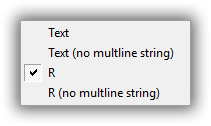
\includegraphics[scale=0.50]{./res/menu_r_rterm_highlighter_io.png}\\

\begin{scriptsize}\begin{tabularx}{\textwidth}{>{\hsize=0.3\hsize}X>{\hsize=0.7\hsize}X}\\
    \hline
    \textbf{Option} & \textbf{Description} \\
    \hline
    Text & Sets the IO highlighter to Text \\
    Text (no multline string) & Sets the IO highlighter to Text without string multline suport \\
    R & Sets the IO highlighter to R \\
    R (no multline string) & Sets the IO highlighter to R without string multline suport \\
    \hline
  \end{tabularx}\end{scriptsize}


\hypertarget{menu_r_rterm_highlighter_Log}{}
\subsubsection{Highlighter LOG}\\
\index{R menu!Rterm highlighter LOG}

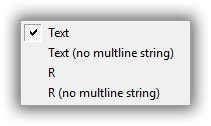
\includegraphics[scale=0.50]{./res/menu_r_rterm_highlighter_log.png}\\

\begin{scriptsize}\begin{tabularx}{\textwidth}{>{\hsize=0.3\hsize}X>{\hsize=0.7\hsize}X}\\
    \hline
    \textbf{Option} & \textbf{Description} \\
    \hline
    Text & Sets the LOG highlighter to Text \\
    Text (no multline string) & Sets the LOG highlighter to Text without string multline suport \\
    R & Sets the LOG highlighter to R \\
    R (no multline string) & Sets the LOG highlighter to R without string multline suport \\
    \hline
  \end{tabularx}\end{scriptsize}


\newpage
\hypertarget{menu_r_rterm_linewrap}{}
\subsubsection{Line wrap}\\
\index{R menu!Rterm line wrap}

\includegraphics[scale=0.50]{./res/menu_r_rterm_linewrap.png}\\

\begin{scriptsize}\begin{tabularx}{\textwidth}{>{\hsize=0.3\hsize}X>{\hsize=0.7\hsize}X}\\
    \hline
    \textbf{Option} & \textbf{Description} \\
    \hline
    IO & Sets line wrap to IO \\
    LOG & Sets line wrap to LOG \\
    \hline
  \end{tabularx}\end{scriptsize}


\hypertarget{menu_r_rterm_history}{}
\subsubsection{History}\\
\index{R menu!Rterm history}

\includegraphics[scale=0.50]{./res/menu_r_rterm_history.png}\\

\begin{scriptsize}\begin{tabularx}{\textwidth}{>{\hsize=0.3\hsize}X>{\hsize=0.7\hsize}X}\\
    \hline
    \textbf{Option} & \textbf{Description} \\
    \hline
    Save & Saves the history \\
    Load & Loads the history \\
    Prior & Prior section of the history \\
    Next & Next section of the history \\
    \hline
  \end{tabularx}\end{scriptsize}


\hypertarget{menu_r_rterm_workspace}{}
\subsubsection{Workspace}\\
\index{R menu!Rterm workspace}

\includegraphics[scale=0.50]{./res/menu_r_rterm_workspace.png}\\

\begin{scriptsize}\begin{tabularx}{\textwidth}{>{\hsize=0.3\hsize}X>{\hsize=0.7\hsize}X}\\
    \hline
    \textbf{Option} & \textbf{Description} \\
    \hline
    Save & Saves the workspace \\
    Load & Loads the workspace \\
    \hline
  \end{tabularx}\end{scriptsize}


\hypertarget{menu_r_rterm_fontsize}{}
\subsubsection{Font of active control (not permanent)}\\
\index{R menu!Rterm fontsize}

\includegraphics[scale=0.50]{./res/menu_fontsize_generic.png}\\

\begin{scriptsize}\begin{tabularx}{\textwidth}{>{\hsize=0.3\hsize}X>{\hsize=0.7\hsize}X}\\
    \hline
    \textbf{Option} & \textbf{Description} \\
    \hline
    Increase & Increase the font size \\
    Decrease & Decrease the font size \\
    \hline
  \end{tabularx}\end{scriptsize}


\hypertarget{menu_r_send}{}
\subsection{Send}
\index{R menu!send}

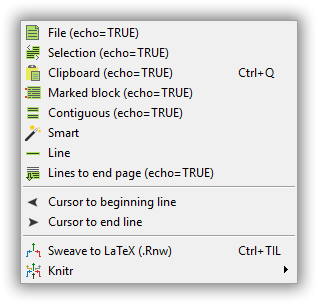
\includegraphics[scale=0.50]{./res/menu_r_send.png}\\

\begin{scriptsize}\begin{tabularx}{\textwidth}{>{\hsize=0.5\hsize}X>{\hsize=0.7\hsize}X}\\
    \hline
    \textbf{Option} & \textbf{Description} \\
    \hline
    File & Sends current file to R interpreter \\
    Selection & Sends current selection to R interpreter \\
    Marked block & Sends current marked block to R interpreter \\
		  Contiguous & Sends contiguous lines to R interpreter \\
    Smart & Sends complete instruction blocks when the cursor is located in a complex context \\
    Line & Sends current line to R interpreter echoing it \\
    Lines to end page & Sends all visible lines to end page echoing it \\
    Cursor to beginning line & Sends cursor position to beginning line \\
    Cursor to end line & Sends cursor position to end line \\
    Sweave & Sends to R interpreter \texttt{Sweave('Active file')} instruction \\
    Knitr & \textit{\htmladdnormallink{See options ...}{\#menu\_r\_send\_knitr}} \\
    \hline
  \end{tabularx}\end{scriptsize}

\hypertarget{menu_r_send_knitr}{}
\subsubsection{Knitr}\\
\index{Knitr}

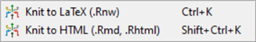
\includegraphics[scale=0.50]{./res/menu_r_send_knitr.png}\\

\begin{scriptsize}\begin{tabularx}{\textwidth}{>{\hsize=0.3\hsize}X>{\hsize=0.7\hsize}X}\\
    \hline
    \textbf{Option} & \textbf{Description} \\
    \hline
    Knit to LaTeX (Rnw) & Knit the *.Rnw file to \LaTeX \\
    Knit to HTML (Rmd, Rhtml) & Knit the *.Rmd or *.Rhtml file to HTML\\
    \hline
  \end{tabularx}\end{scriptsize}


\hypertarget{menu_r_control}{}
\subsection{Control}
\index{R menu!control}

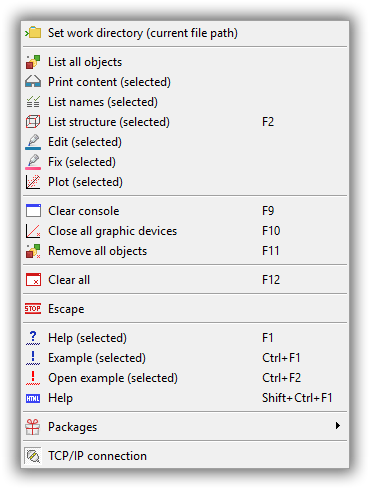
\includegraphics[scale=0.50]{./res/menu_r_control.png}\\

\begin{scriptsize}\begin{tabularx}{\headwidth}{>{\hsize=0.4\hsize}X>{\hsize=0.7\hsize}X}\\
    \hline
    \textbf{Option} & \textbf{Description} \\
    \hline
    Work directory (get/set) &  \textit{\htmladdnormallink{See options ...}{\#menu\_r\_control\_workdir}} \\
    List all objects & Sends to R interpreter a \texttt{ls()} instruction \\
    Print content (selected) & Sends to R interpreter a \texttt{selected} word \\
    List names (selected) & Sends to R interpreter a \texttt{names(selected)} instruction \\
    List structure (selected) & Sends to R interpreter a \texttt{str(selected)} instruction \\
    Edit (selected) & Sends to R interpreter a \texttt{edit(selected)} instruction \\
    Fix (selected) & Sends to R interpreter a \texttt{fix(selected)} instruction \\
    Plot (selected) & Sends to R interpreter a \texttt{plot(selected)} instruction \\
    Clear console & Sends and executes the virtual \texttt{CTRL + L} (clear screen) instruction \\
    Close all graphic devices & Sends to R interpreter a \texttt{graphics.off()} instruction \\
    Remove all objects & Sends to R interpreter a \texttt{rm(list=ls())} instruction \\
    Clear all & Sends to R interpreter a \texttt{graphics.off()}; \texttt{rm(list=ls())} \texttt{CTRL + L} instructions \\
    Escape & Stops all computations in Rgui \\
    Help (selected) & Sends to R interpreter a \texttt{help(selected)} instruction \\
    Example (selected) & Sends to R interpreter a \texttt{example(selected)} instruction \\
    Open example (selected) & Sends to R interpreter an instruction to generate an example text file of the \texttt{object selected}\\
    Help & Sends to R interpreter a \texttt{help.start(update=FALSE)} instruction \\
    Packages & \textit{\htmladdnormallink{See options ...}{\#menu\_r\_control\_packages}} \\
    TCP/IP connection & Sends to R interpreter an instruction to start: \texttt{startSocketServer(port=portnumber)} or stop: \texttt{startSocketServer(port=portnumber)} the TCP/IP connection \\
    \hline
  \end{tabularx}\end{scriptsize}


\newpage
\hypertarget{menu_r_control_workdir}{}
\subsubsection{Work directory}\\
\index{Work directory}
\index{getwd()}
\index{setwd()}
\index{R menu!work directory}

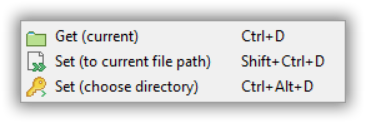
\includegraphics[scale=0.50]{./res/menu_r_control_workdir.png}\\

\begin{scriptsize}\begin{tabularx}{\headwidth}{>{\hsize=0.2\hsize}X>{\hsize=0.7\hsize}X}\\
    \hline
    \textbf{Option} & \textbf{Description} \\
    \hline
    Get (current) & Get the work directory of the R interpreter \\
    Set (to current file path) & Set the work directory of the R interpreter to the current file path \\
    Set (choose) & Set the work directory of the R interpreter allowing to choose from the Windows dialog \\
    \hline
  \end{tabularx}\end{scriptsize}

\hypertarget{menu_r_control_packages}{}
\subsubsection{Packages}\\
\index{R menu!control packages}

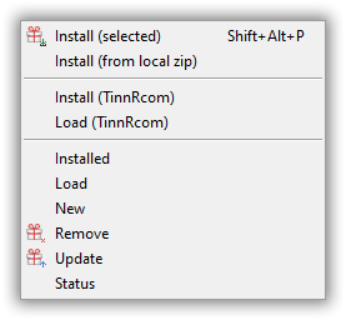
\includegraphics[scale=0.50]{./res/menu_r_control_packages.png}\\

\begin{scriptsize}\begin{tabularx}{\headwidth}{>{\hsize=0.2\hsize}X>{\hsize=0.7\hsize}X}\\
    \hline
    \textbf{Option} & \textbf{Description} \\
    \hline
    Install & Sends to R interpreter an \texttt{utils:::menuInstallPkgs()} instruction \\
    Install (from local zip) & Sends to R interpreter a \texttt{utils:::menuInstallLocal()} instruction \\
    Install (TinnRcom) & Sends to R interpreter instruction to install TinnRcom package and its dependecies.
      By default it is not necessary since the TinnRcom package is automatically installed \\
    Load (TinnRcom) & Sends to R interpreter an \texttt{library(TinnRcom)} instruction.
      By default it is not necessary since the TinnRcom package is automatically loaded when R starts \\
    Installed & Sends to R interpreter a \texttt{installed.packages()} instruction \\
    Load & Sends to R interpreter a \texttt{local(\{pkg $<$- select.list(sort(.packages(all.available = TRUE))); if(nchar(pkg)) library(pkg, character.only=TRUE)\})} instruction \\
    New & Sends to R interpreter a \texttt{new.packages()} instruction \\
    Remove & Sends to R interpreter a \texttt{local(\{pkg $<$- select.list(sort(.packages(all.available = TRUE))); if(nchar(pkg)) remove.packages(pkg)\})} instruction \\
    Update & Sends to R interpreter an \texttt{update.packages(ask='graphics')} instruction \\
    Status & Sends to R interpreter a \texttt{packageStatus()} instruction \\
    \hline
  \end{tabularx}\end{scriptsize}
